\section{Newton's Method}

Excessive coordinates - freebody diagrams in \autoref{fig:freeBodyCart} and \ref{fig:freeBodyPendulum}

\begin{figure}[H]
  \hspace{-10pt}
  \captionbox
  {
    freeBodyCart
    \label{fig:freeBodyCart}
  }
  {
    \hspace{-1cm}
    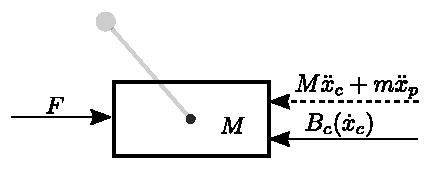
\includegraphics[width=.4\textwidth]{figures/freeBodyCart}
  }
  \hspace{20pt}
  \captionbox 
  {
    freeBodyPendulum
    \label{fig:freeBodyPendulum}
  }
  {
    \hspace{-1cm}
    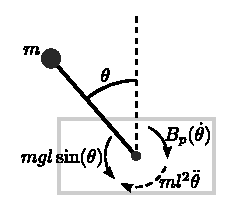
\includegraphics[width=.28\textwidth]{figures/freeBodyPendulum}
  }  
\end{figure}
%
Newton's second law for the cart along $x_c$. Freebody diagram in \autoref{fig:freeBodyCart}
\begin{flalign}
  M\ddot{x}_c + m\ddot{x}_p &= F - B_c(\dot{x}_c) &
  \label{eq:newtonAlongX}
\end{flalign}
%
Applying Newton's second law for rotational motion. Freebody diagram in \autoref{fig:freeBodyPendulum}
\begin{flalign}
  ml^2 \ddot{\theta} &= mgl \sin \theta - B_p(\dot{\theta}) &
  \label{eq:newtonRotation}
\end{flalign}
%
Relation of D'alumbert forces for the pendulum decomposed as tangential forces,
\begin{flalign}
  - m\ddot{x}_p \cos \theta - m\ddot{y}_p \sin \theta &= ml \ddot{\theta} &
  \label{eq:dalumbert}
\end{flalign}
%
To combine \autoref{eq:dalumbert} and \ref{eq:newtonRotation}, \autoref{eq:dalumbert} is written as torques,
\begin{flalign}
  - ml\ddot{x}_p \cos \theta - ml\ddot{y}_p \sin \theta &= ml^2 \ddot{\theta} &
  \label{eq:dalumbertTorques}
\end{flalign}
%
\autoref{eq:dalumbert} and \ref{eq:newtonRotation} are combined,
\begin{flalign}
  - ml\ddot{x}_p \cos \theta - ml\ddot{y}_p \sin \theta &=  mgl \sin \theta - B_p(\dot{\theta}) &
  \label{eq:dalumbertTorquesANDnewtonRotation}
\end{flalign}
%
The system dynamics is then represented using excessive coordinates by the following set of equations:
\begin{flalign}
  \begin{cases}
    - ml\ddot{x}_p \cos \theta - ml\ddot{y}_p \sin \theta =  mgl \sin \theta - B_p(\dot{\theta}) & \\
    M\ddot{x}_c + m\ddot{x}_p = F - B_c(\dot{x}_c) &
  \end{cases}  & \unit{\cdot}
  \label{eq:excessiveCoordinates}
\end{flalign}
%
Writing the excessive coordinates, \autoref{fig:excessiveCoordinates}, in therms of the generalized coordinates, \autoref{fig:mechanicalDrawing},
\begin{flalign}
  \begin{cases}
    x_c &=  x  \\
    y_c &=  0  
  \end{cases} &
    \hspace{20pt}
  \begin{cases}
    x_p =  x - l\sin \theta \\
    y_p =  l\cos \theta
  \end{cases}  &
  \label{eq:coordinateTransformation}
\end{flalign}
%
Finding the derivatives for the transformation,
\begin{flalign}
  \begin{cases}
    \dot{x}_p &= \dot{x} - l\cos \theta \dot{\theta} \\
    \dot{y}_p &= -l\sin \theta \dot{\theta}
  \end{cases} &
    \hspace{20pt}
  \begin{cases}
    \ddot{x}_p = \ddot{x} + l \sin \theta \dot{\theta}^2 - l\cos \theta \ddot{\theta} \\
    \ddot{y}_p = -l\cos \theta \dot{\theta}^2  -l\sin \theta \ddot{\theta}
  \end{cases}  &
  \label{eq:transformationDerivatives}
\end{flalign}
%
Rewriting \autoref{eq:excessiveCoordinates} in generalized coordinates using the cooredinate transformation from \autoref{eq:coordinateTransformation} and \ref{eq:transformationDerivatives} yields,
\begin{flalign}
  \begin{cases}
     - ml( \ddot{x} + l \sin \theta \dot{\theta}^2 -l\cos \theta \ddot{\theta} ) \cos \theta - ml ( -l \cos \theta \dot{\theta}^2 -l\sin \theta \ddot{\theta} ) \sin \theta =  mgl \sin \theta - B_p(\dot{\theta}) & \\
     M\ddot{x} + m( \ddot{x} + l\sin \theta \dot{\theta}^2 - l \cos \theta \ddot{\theta} ) = F - B_c(\dot{x}) &
  \end{cases} && \nonumber
\end{flalign}
\vspace{-14pt}
\begin{flalign}
  \begin{cases}
   ml^2 \ddot{\theta} - ml\cos \theta \ddot{x} - mgl \sin \theta &= - B_p(\dot{\theta}) \\
  ( M + m ) \ddot{x} + ml\sin \theta \dot{\theta}^2 - ml\cos \theta \ddot{\theta} &= F - B_c(\dot{x})  \ \ \ \ ,
\end{cases} & \unit{\cdot}
\label{eq:generalizedCoordinates}
\end{flalign}
%
which is the final dynamic equations for the cart pendulum system.